Ex3 give us that the temperature and density of air difference are constant so it means that $\Dot{CO2_{Air}}$ and $\Dot{CO2_{Top}}$ depend on data of CO2 concentration. However, when we did some test with data, results were almost approximately same as the first time we have done.

Follow the constant variables as the exercise 2.b above, dx and constant temperature and density of air difference as below:

\textbf{
p\_Air = 3;
p\_Top = 2.987;
T\_Air = 295;
T\_Top = 291;
T\_Out = 288.9;
}

\begin{figure}[h]
\centering
    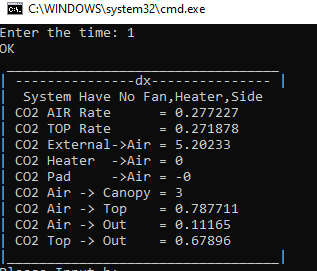
\includegraphics[width = 3in, height = 3in]{Code/Pic/result.png}
    \caption{Output}
    \label{fig:my_label}
\end{figure}

Note: There is NO Heater, NO Fan and NO sidewalls CO2 emission so that $CO2_{Heater->Air}$ and  $CO2_{Pad->Air}$ are 0 but there are still leakages on sidewalls so that $CO2_{Air->Out}$ still has a non-zero value.

